\documentclass[conference]{IEEEtran}
\RequirePackage{cite}
\RequirePackage{amsmath,amssymb,amsfonts}
\RequirePackage{physics}
\RequirePackage{algorithmic}
\RequirePackage{graphicx}
\RequirePackage{textcomp}
\RequirePackage{xcolor}
\RequirePackage{hyperref}
\RequirePackage{csquotes}
\RequirePackage{listings}
\RequirePackage{siunitx}

\RequirePackage{xcolor}
\definecolor{officeblue}{RGB}{53, 136, 195}
\setkeys{Gin}{width=0.4\textwidth}
\def\BibTeX{{\rm B\kern-.05em{\sc i\kern-.025em b}\kern-.08em
    T\kern-.1667em\lower.7ex\hbox{E}\kern-.125emX}}
    
    
\newcommand{\Sim}{\lstinline{stda-sailboat-simulator}\ }
\newcommand{\Casadi}{\lstinline{CasADi}\ }
\begin{document}
\title{Simulated Control and Path Planning of an Autonomous Sailboat}
\author{Andrew~Fearing, Neelay~Junnarkar,  Hamza~Kamran~Khawaja}
\maketitle


\begin{abstract}
In this project we develop a planning and control method for a sailboat to maneuver autonomously, in the presence of obstacles, to a high level target described in \(x, y\) coordinates. We test our method in the \Sim against various wind directions and with and without presence of waves. 
\end{abstract}


\section{Introduction}
Wind-propelled sailing is a complex task. The sailboat is entirely dependent on the wind and water for propulsion and steering. In addition, boats are subject to environmental disturbances such as wind gusts, water currents, and waves. Because of this, autonomous sailing presents an interesting problem in robotics.

Sailboats have the potential to go on long-term missions at sea. They need actuators only for the rudder and sail, and so they can be solar powered. Possible uses include plastic waste collection, coastal surveillance, and long-term data collection.

In this paper, we present an application of an optimization-based path planner to successfully navigate the simulated sailboat to a target position in the presence of obstacles and under different environmental conditions. In particular, we demonstrate the sailboat succesfully traversing a narrow channel. The sailboat dimensions, kinematics, and dynamics model is given in \cite{Buehler2018}. Our approach uses a simple PID controller for rudder control. The sail angle for propulsion is set using a closed-form function of the apparent wind angle.

% \begin{figure}
%     \centering
%     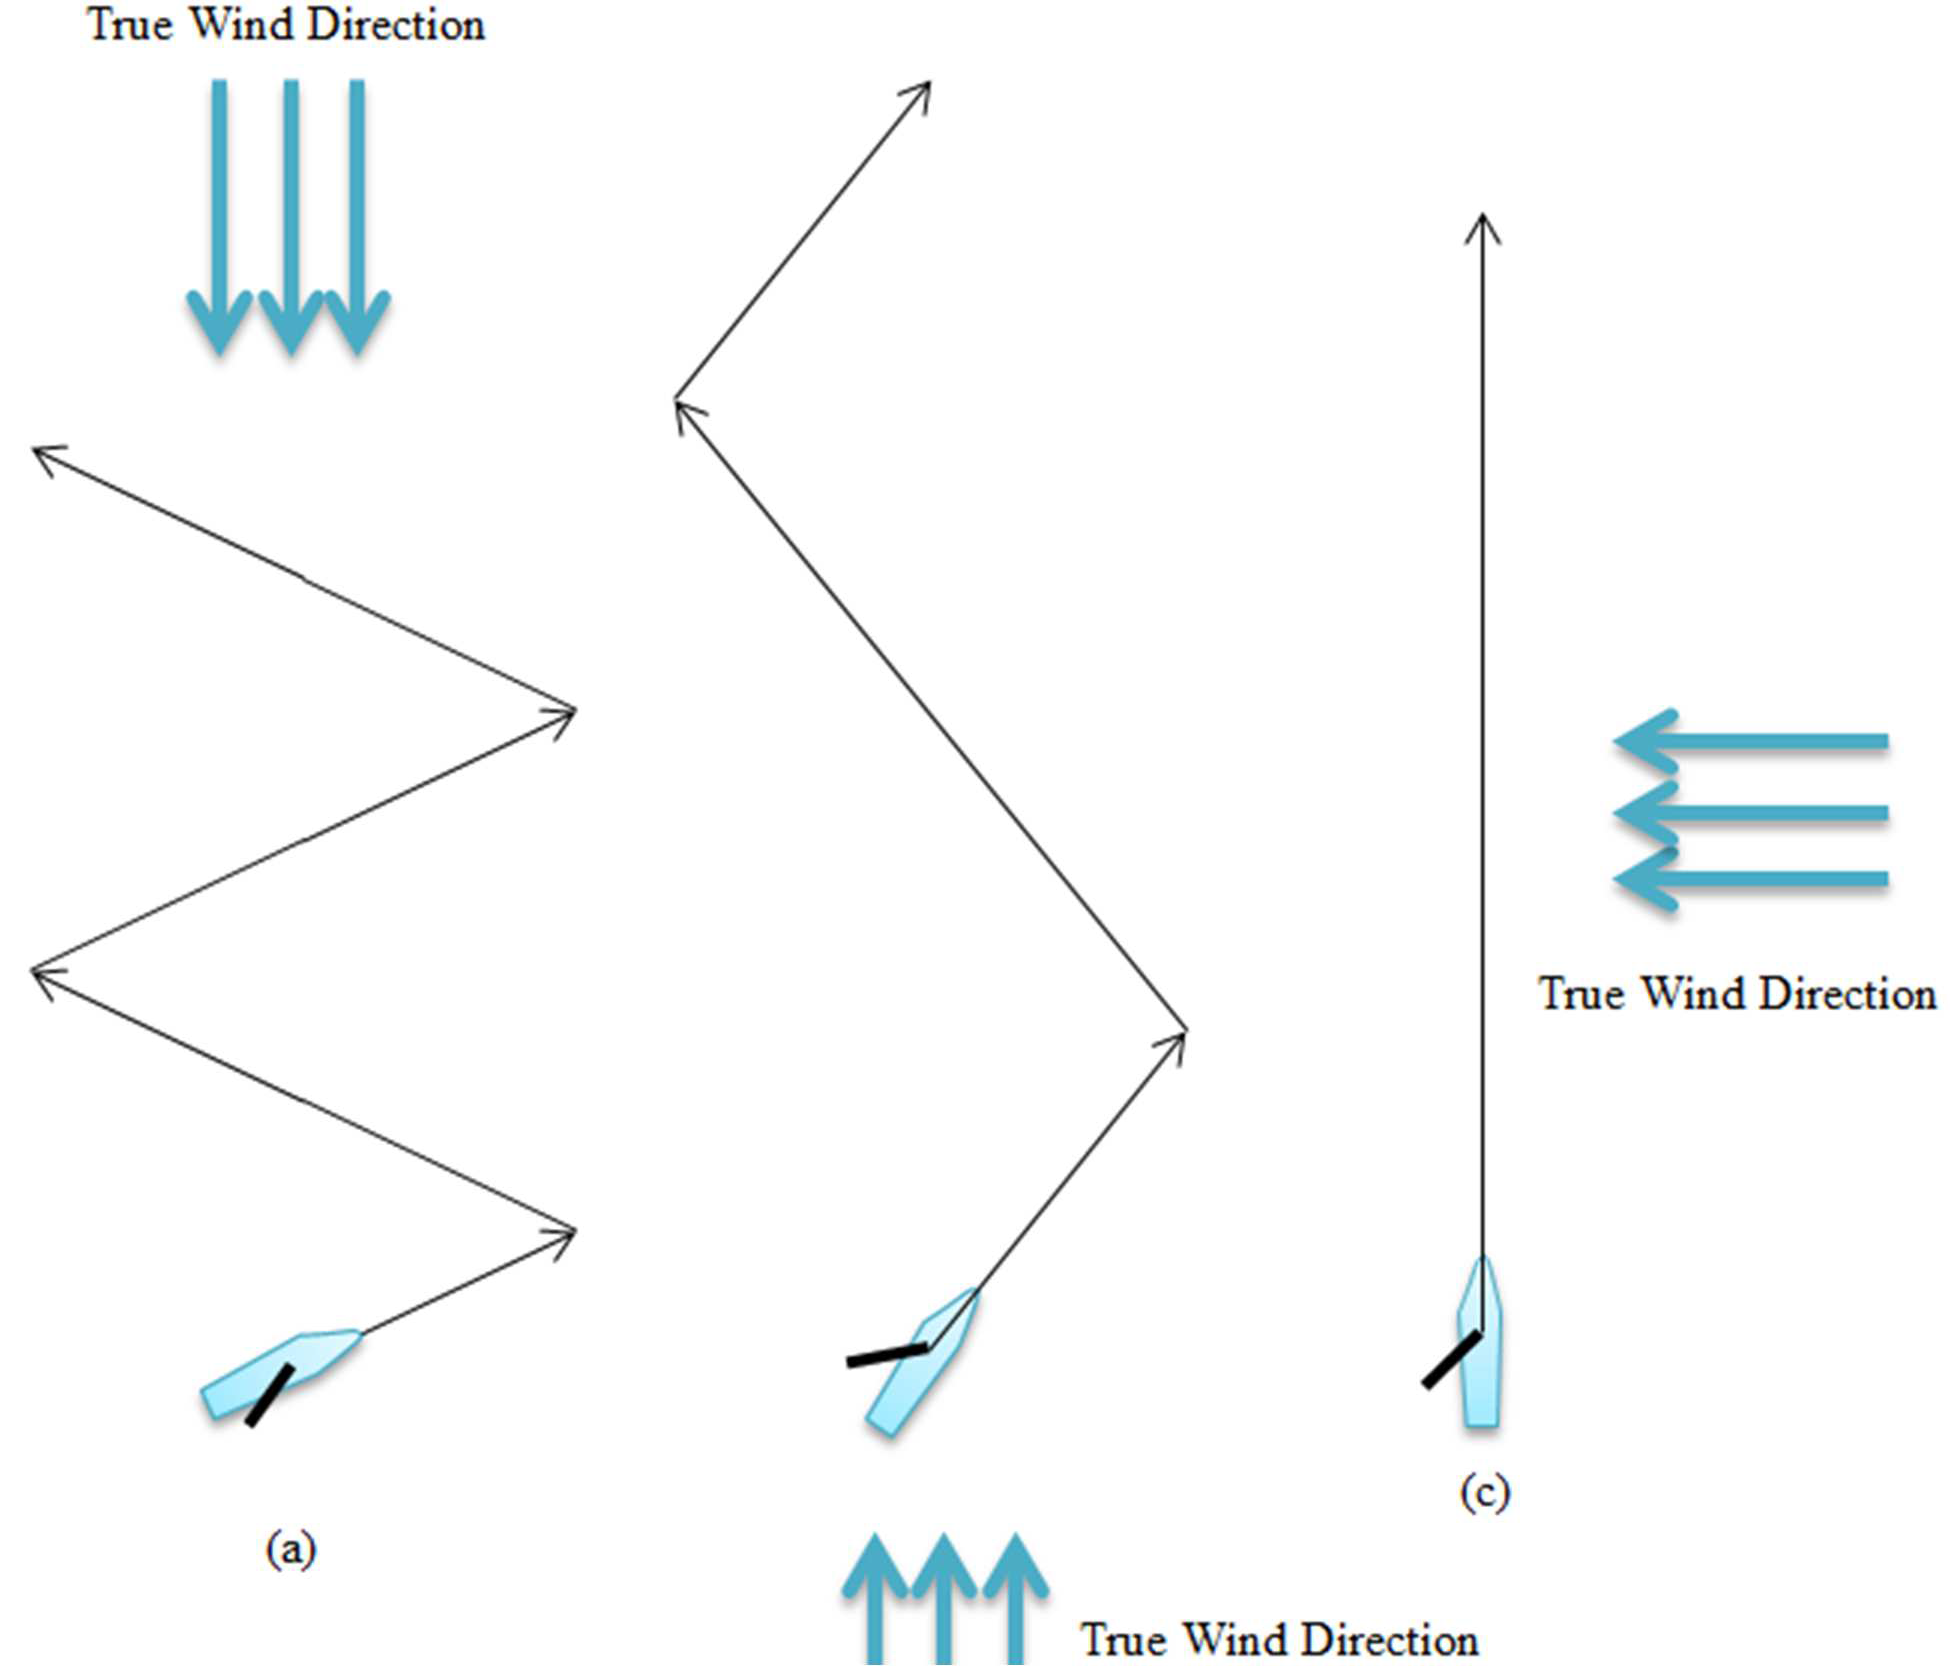
\includegraphics{documents/figures/alves_modes.png}
%     \caption{Modes of sailing \cite{Alves2010}}
%     \label{fig:alves_modes}
% \end{figure}
% \begin{figure}
%     \centering
%     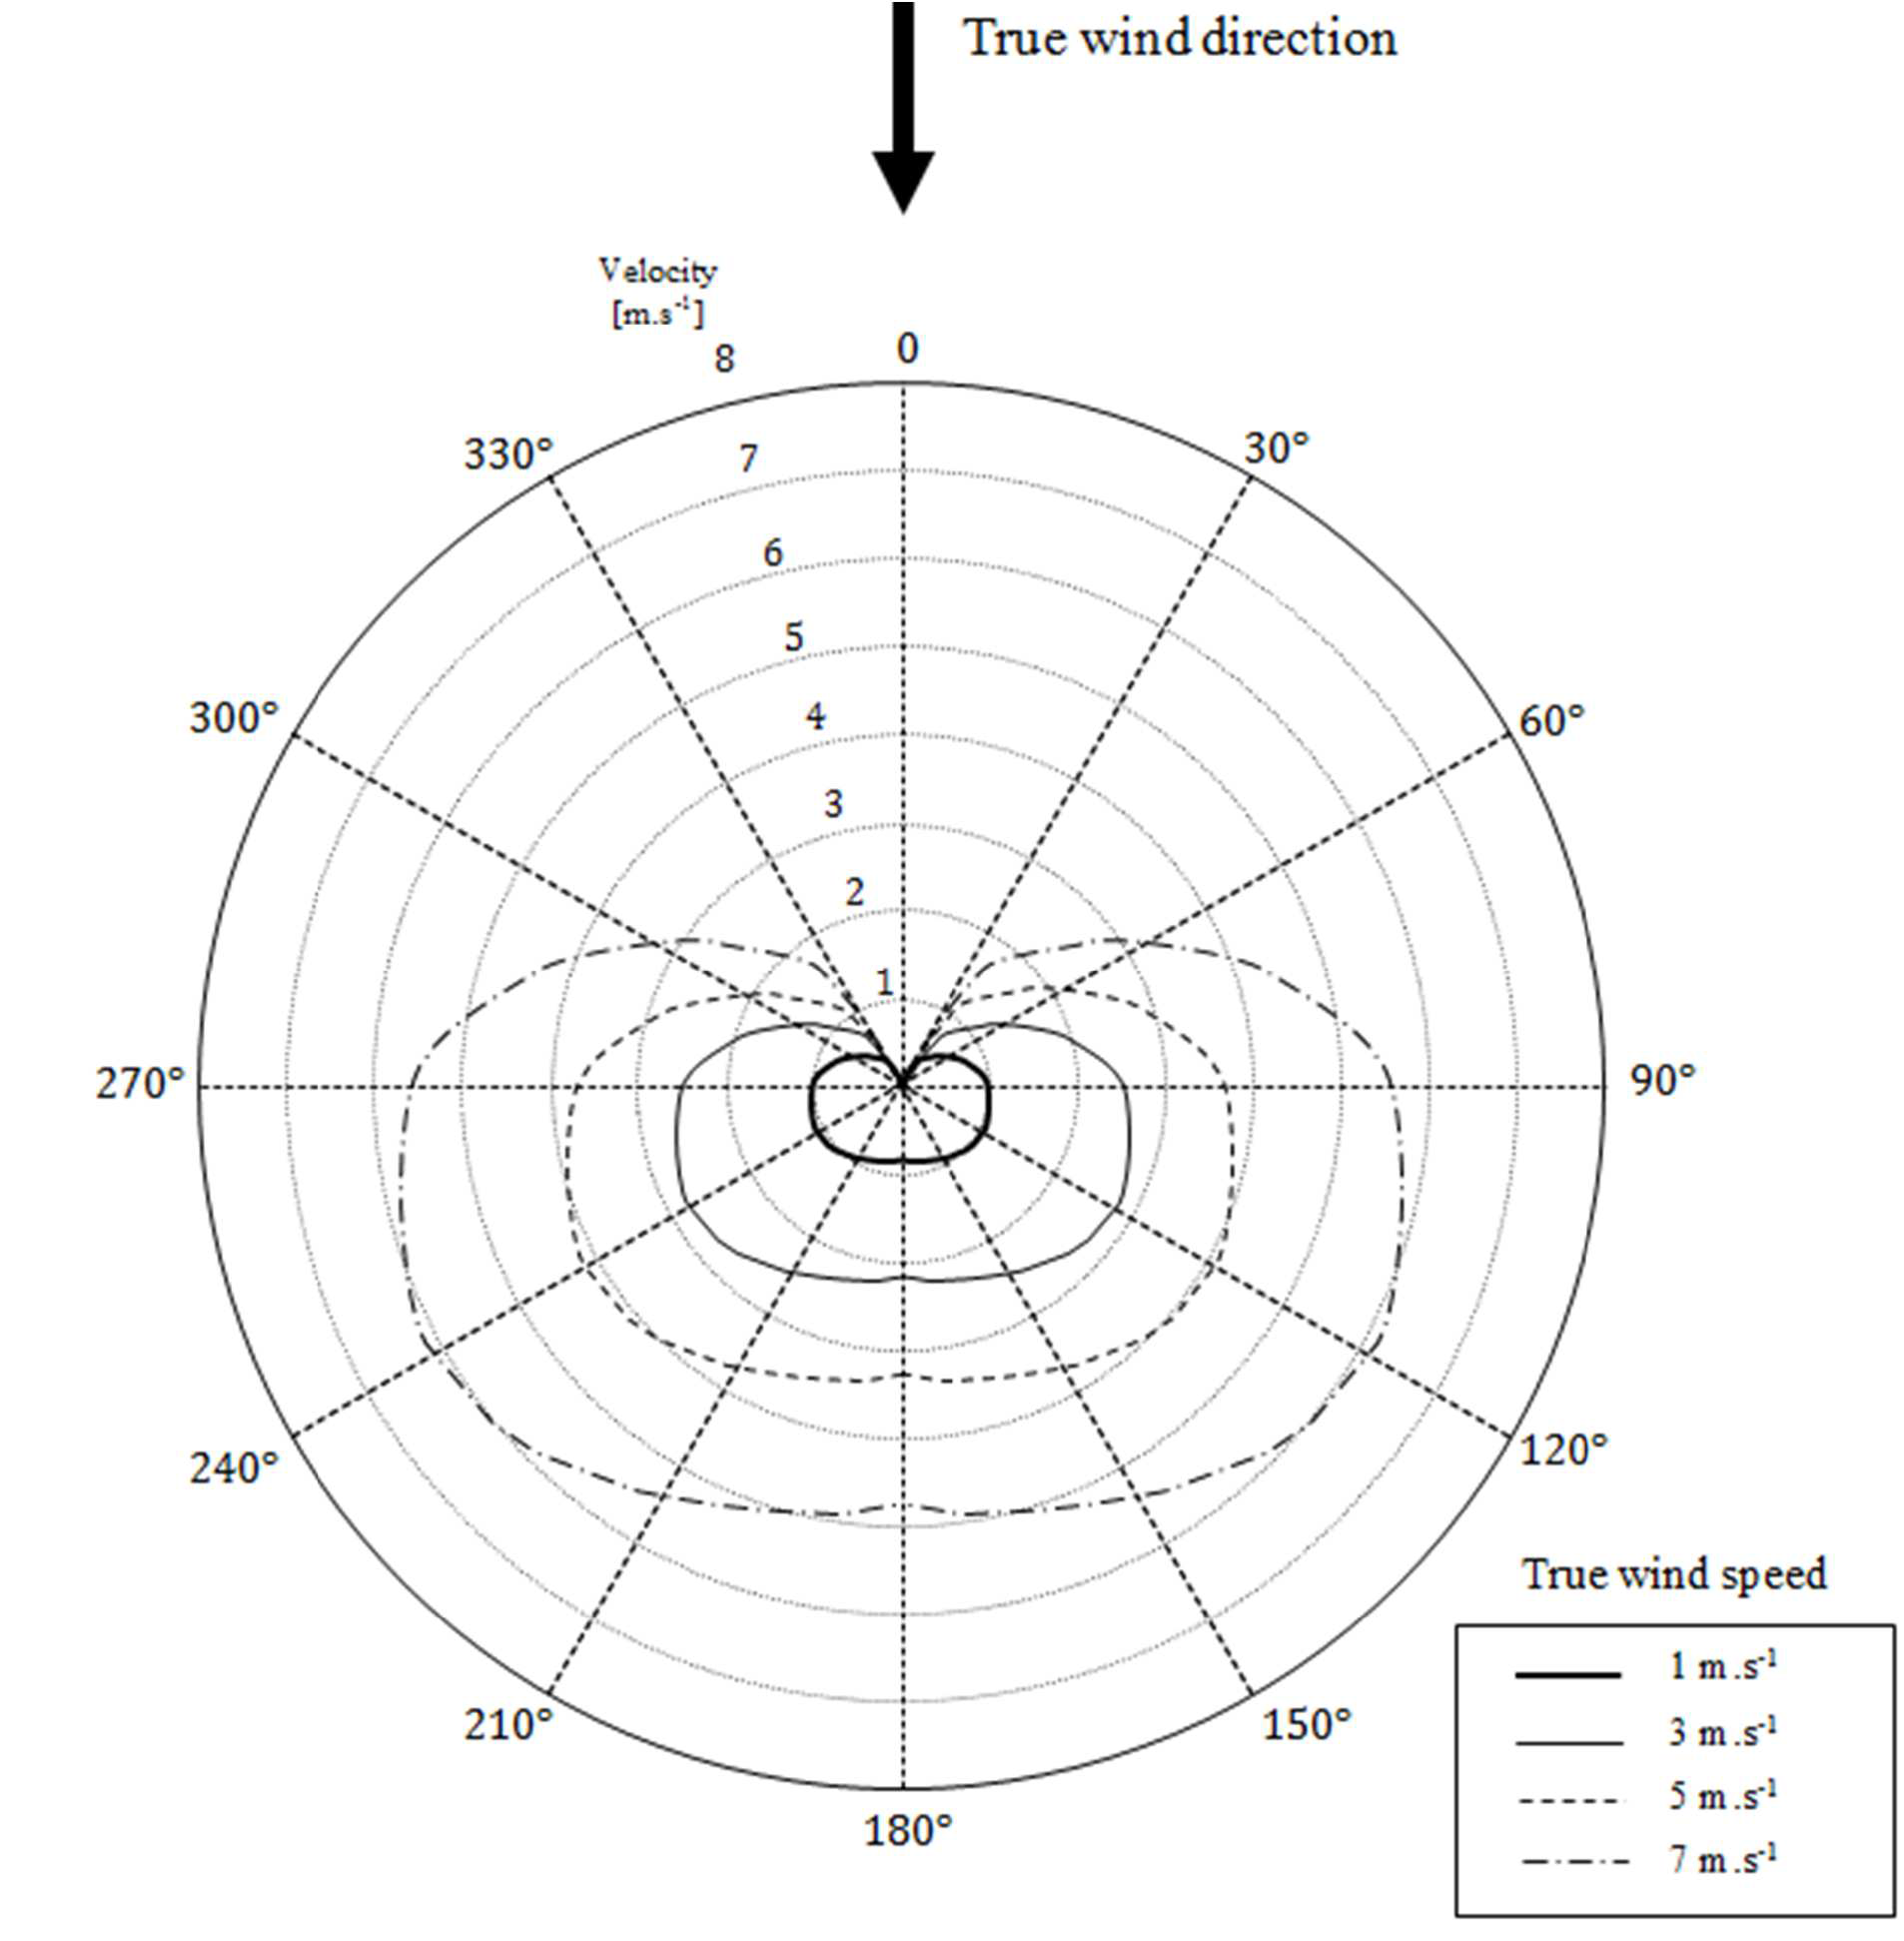
\includegraphics{documents/figures/alves_vpp.png}
%     \caption{Velocity polar diagram \cite{Alves2010}}
%     \label{fig:alves_velocity}
% \end{figure}
% \subsection{Related Work}


\section{Related Work}
Interest in autonomous sailboats has grown over the past decade. There are several different areas of research in pursuit of sailing USV's, including propulsion, control, navigation , and simulation.


% \cite{Cruz2010, Erckens2010, Xiao2014, Santos2016, Santos2018, HelmiAbrougui2019}

Previous research in model-based sailboat control have used PID controllers for heading, such as in \cite{Cruz2010, Erckens2010}. \cite{Xiao2014} used a nonlinear heading controller using the integrator backstepping method. \cite{Santos2018} used a lookup table of PI parameters to suit the control requirements of different environmental conditions.

Efforts in propulsion research \cite{Saoud2015, Setiawan2019, DosSantos2020} focus on optimizing the sail angle and shape. There are several criteria that can be evaluated, such as time to target, energy consumption, safety, and aerodynamic forces.

% path planning \cite{Sauze2010, Petres2011, Plumet2013}
There are several methods that have been used for autonomous sailboat path planning. A*, theta*, and D* algorithms have previously been successful \cite{Erckens2010}. Path planning using potential fields is promising. They offer a way to unify the navigation factors (goal, obstacles, boat characteristics, costs of maneuvers) into a single framework \cite{Plumet2013}. 

One area of that has not found much attention is robustness to environmental effects. Most of the above mentioned literature use some combination of 3- or 4-DoF simulators and practical experiment on a \SIrange{1}{10}{\meter}-scale sailboat in fair weather. 3- and 4-DoF simulators usually simplify models by neglecting the roll, pitch, and \(z\)-axis motions brought about by waves and wind. Of the open-source USV simulators, the authors were able to find two that support 6-DoF sailboat simulation and model wind, buoyancy, waves, and foil dynamics. \cite{Paravisi2019} demonstrated USVSim, an open-source USV simulator that incorporates Gazebo, the Free-floating Plugin, UWSim, and the LiftDrag Gazebo Plugin. USVSim includes many features, but it is time-consuming to set up the simulation environment. \cite{Buehler2018} presented \Sim, a 6-DoF sailboat simulator written in Python. The simulator uses the RK45 method to solve an ODE over time. Although the simulator does not feature 3D-visualization as Gazebo offers, it requires only a few common Python packages to run.

% \cite{Buehler2018, Paravisi2019, Setiawan2020}





% There are simulations, but few work with sailboats. One of the challenges of simulation is modelling the effects of wind on a boat. \cite{Paravisi2019} demonstrated a USV simulator that models environmental disturbances, including waves, buoyancy, water currents, wind currents, and foil dynamics. This simulator integrates ROS, Gazebo, ..., for simulation and is complicated. Time-consuming environment setup. \cite{Buehler2018} demonstrated \Sim in Python. The simulator uses RK45 method to solve an ODE over time. The simulator models a 6 DOF rigid body sailboat. \Sim models a constant wind vector and consistent wave sizes.

%The sailboat model kinematics and dynamics are described in \cite{Buehler2018}.



\section{Methods}
\subsection{Simulation setup}
We decided to use the \lstinline{stda-sailboat-simulator} for simplicity, although it required significant 
refactoring of the code base to be in a useable form.

\begin{figure}
    \centering
    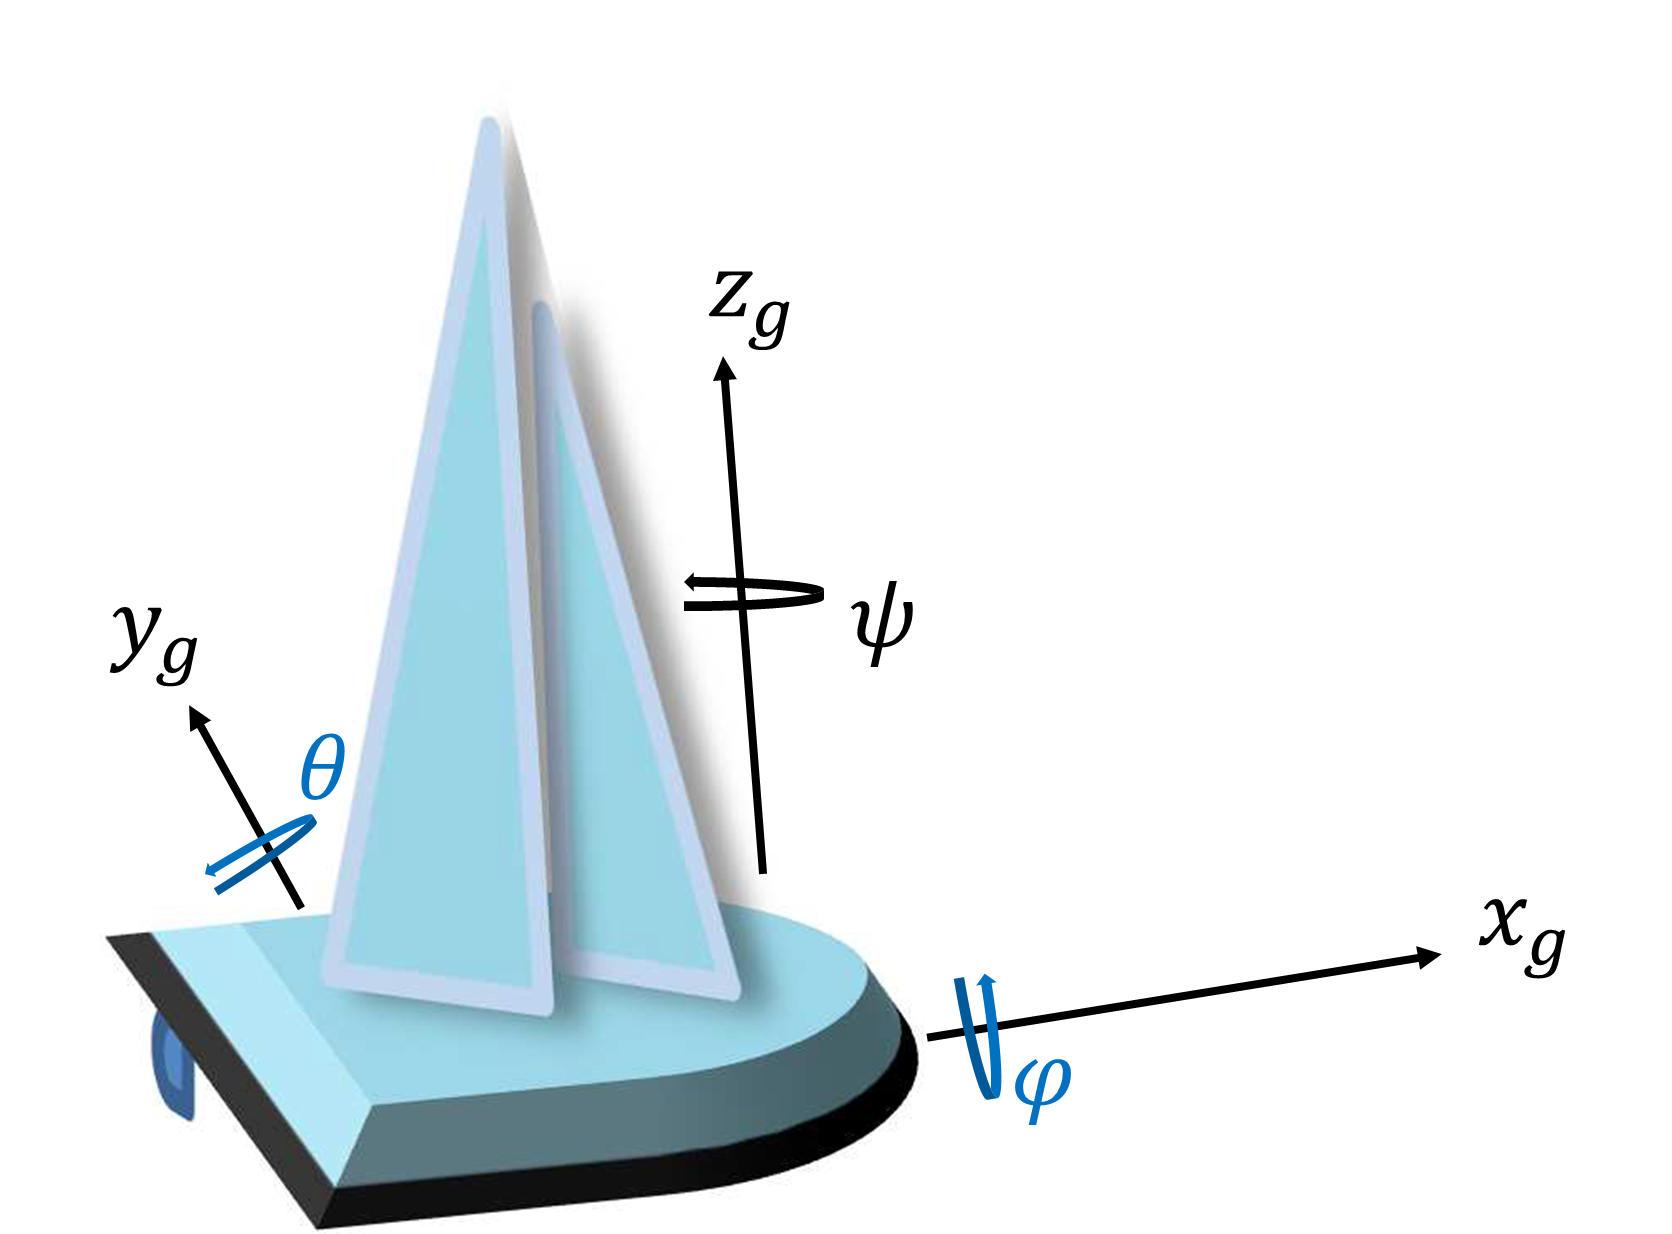
\includegraphics{documents/figures/alves_boat_with_buehler_axes.png}
    \caption{Sailboat axes~\cite{Alves2010}}
    \label{fig:sailboat_components}
\end{figure}
\begin{table}
    
    \centering
    \begin{tabular}{ccc}
    name & position & velocity \\
     &\(x_g\) & \(v_x\) \\
     &\(y_g\) & \(v_y\) \\
     &\(z_g\) & \(z_x\) \\
     heading&\(\psi\) & \(p\) \\
     \textcolor{officeblue}{roll} & \textcolor{officeblue}{\(\theta\)} & \textcolor{officeblue}{\(q\)} \\
     \textcolor{officeblue}{pitch}&\textcolor{officeblue}{\(\varphi\)} & \textcolor{officeblue}{\(r\)} \\
     \textcolor{officeblue}{rudder angle} & \textcolor{officeblue}{\(\rho\)} & \\
     \textcolor{officeblue}{sail angle}   & \textcolor{officeblue}{\(\gamma\)} & 
    \end{tabular}
    \caption{The 14 sailboat state variables~\cite{Buehler2018}.}
    \label{tab:state_vars}
\end{table}

\subsection{Feedback Loop}

Our control design modularizes the system into two stages: a planner, which takes in high level \(x,y\) position 
targets and generates heading trajectories, and a yaw controller, which generates sail and rudder angles 
to track the reference heading trajectory output by the planner. Since the planning stage does not need 
to be run at the same rate as the yaw controller due to the slow speed of the boat, we create an inner feedback loop between the yaw controller and the system dynamics, and an outer feedback loop that incorporates the planner and is run at a lower rate. See Figure \ref{fig:controller_block_diagram} for a block diagram.

\begin{figure}
    \centering
    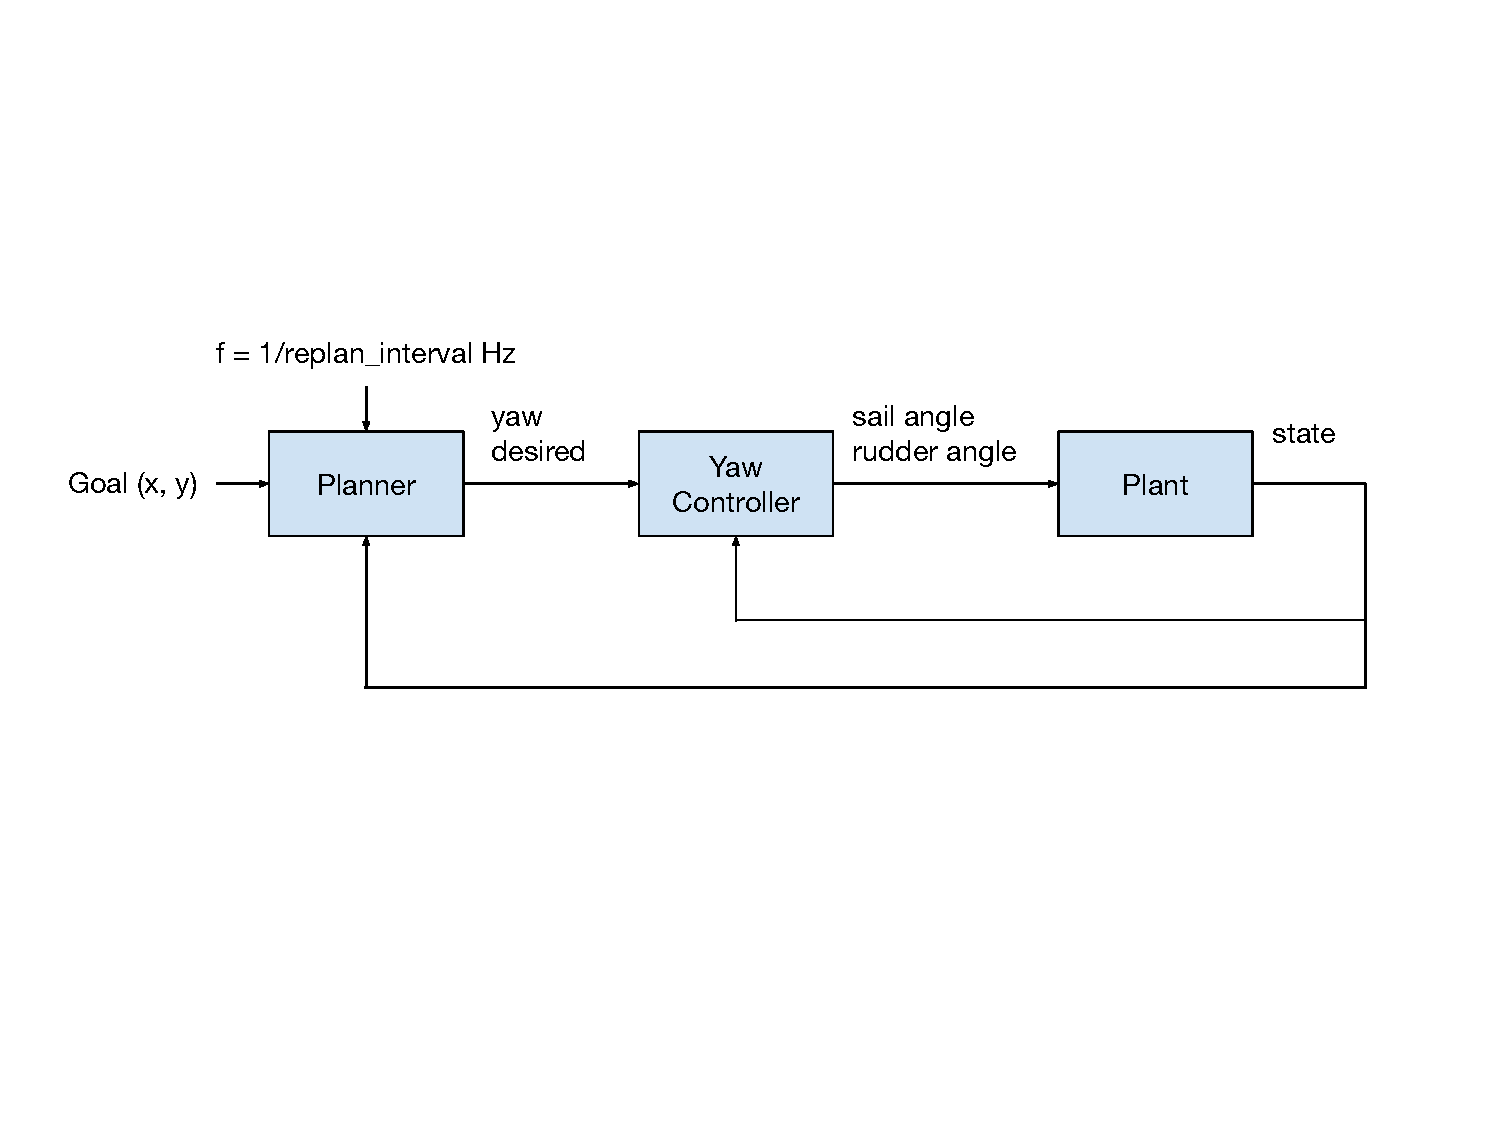
\includegraphics[trim={1.1cm 7cm 2cm 5cm},clip]{documents/final_pres_figs/controller_block_diagram.pdf}
    \caption{Block diagram of planner and controller}
    \label{fig:controller_block_diagram}
\end{figure}

\subsection{Yaw Controller}

The yaw controller is input the full boat state and outputs the rudder and sail angles to set on the boat to track the reference heading trajectory from the planner. Note that in the boat dynamics model, the rudder and sail angles are related to the rudder and sail angle inputs through a first order system that simulates delays, but for brevity we will refer to the outputs of the yaw controller as the rudder and sail angles of the boat.

We implemented the yaw controller as from \cite{Buehler2018}.
This controller leverages the fact that there is an optimal angle for the sail based on wind direction to decouple the rudder and sail angle controls. The sail angle is given by Eq.~\ref{eq:sail_angle}. Note that the full range of this equation is not physically feasible and is clipped to feasible bounds in the model. The rudder angle controller is implemented as a PID controller with gains determined through LQR.

\begin{equation}
    \theta_{\text{sail}} = \frac{\sin(\theta_{aw})}{\cos(\theta_{aw}) + 0.4\cos^2(\theta_{aw})}
    \label{eq:sail_angle}
\end{equation}

\subsection{Path Planner}

The path planner takes in a high level \(x,y\) position target and outputs a heading trajectory that if followed by the boat will bring the boat along a path to the target. We designed our planner as an optimization based planner which repeatedly solves constrained optimization problems with receding horizons. Replanning allows handling of deviations from the planned trajectory. 

Each optimization problem solves for trajectories of an input \(u\) and states \(q\) over the time interval 
\(t_0\), the time at the start of planning, to \(t_f = t_0 + \text{replanning interval}\). The constraints are to start at the start state, evolve the state in such a way that it satisfies boat dynamics. We add additional constraints to bound the input. As an extension to handle simple obstacles, we represent obstacles as circles in \(x, y\) space. Then, the additional constraint is that the distance between the \(x, y\) position of the boat and the center of each obstacle must exceed the radius of each obstacle.

The optimization problem is formulated as in Equation \ref{eq:optimization_problem}, where \(t_0\) is the time at the start of planning, \(t_f\) is \(t_0\) plus the planning horizon, \(u\) is the input as a function of time from \(t=t_0\) to \(t=t_f\), \(q(t)\) is the state of the boat at time \(t\), \(q_{t_0}\) is the state at the start of planning, \(q_{goal}\) is the desired state of the boat, \(u_{max}\) and \(u_{min}\) are bounds on the input \(u\), \(f_{simple}\) is a simplified dynamics model, \(Q\) and \(R\) are tuneable weight matrices, \(q_{o_i}(t)\) is the location of obstacle \(o_i\) at time \(t\), and \(r_i\) is the radius of obstacle \(i\).

\begin{equation}
\begin{array}{rrclc}
\displaystyle \min_{u, q} & \multicolumn{4}{l}{\int_{t_0}^{t_f} \left((q(t)-q_{goal})^T Q (q(t)-q_{goal}) + u^2(t) R \right)\mathrm{dt}} \\
\mathrm{s.t.} & q(t_0) & = & q_{t_0} &\\
& \dot{q}(t) & = & f_{simple}(q(t), u(t)) & \forall t\\
& \|q(t) - q_{o_i}(t)\|^2 & \geq & r_i^2 & \forall t, i\\
& u(t) & \leq & u_{max} & \forall t\\
& u(t) & \geq & u_{min} & \forall t
\end{array}
\label{eq:optimization_problem}
\end{equation}

Ideally, \(f_{simple}\) would equal the actual dynamics model of the sailboat. However, the dynamics model of the sailboat is large, with 14 state variables, and complicated, with many nonlinear dynamics and involving forces from environmental disturbances not known at the time of planning. Using the real dynamical model would slow down planning, so we instead devise a simplified dynamical model to make the planning efficient \cite{Andersson2018}.

The simplified model we design has three boat states: \(x, y, \psi\) where \(x, y\) are position and \(\psi\) is heading (yaw). The input \(u\) is a non-physical input. Setting yaw as the integral of the non-physical input \(u\) ensures the yaw trajectory is continuous. Additionally, with this design, constraints on \(u\) allow limiting the rate of change of yaw, giving a tuning factor to make the yaw trajectories designed by the planner more feasible on the actual boat model. See Equation \ref{eq:simplified_dynamics} for the simplified dynamical model.

\begin{equation}
    \dot{q} = f_{simple}(q, u) = \mqty[\dot{x} \\ \dot{y} \\ \dot{\psi}]
        = \mqty[v_x \cos(\psi) - v_y \cos(\psi) \\ 
    v_x \sin(\psi) + v_y\cos(\psi) \\ 
    u]
    \label{eq:simplified_dynamics}
\end{equation}

This dynamical model uses the correct derivatives of \(x\) and \(y\), while assuming any slowly and continuously changing heading is feasible. The variables \(v_x\) and \(v_y\) are the boat velocities in the x and y world frame directions. The speed of the boat is considered to be constant over the course of the planning horizon and equal to the speed at the start of planning. 

The solution to the optimization problem gives a trajectory of states \(q(t)\), from which the yaw trajectory is extracted and passed to the yaw controller.

\section{Implementation}

We used the python \Sim simulator to model the dynamics of the sailboat, and implemented the path planner and yaw controller as feeding inputs to the simulator. The path planner is implemented using \Casadi and the IPOPT solver. To implement Equation \ref{eq:optimization_problem}, we discretized it with a fixed number of steps, discretizing the dynamics constraint as \(q_{i+1} = q_i + \delta_t Df\) where \(\delta_t\) is the discretized step time, and \(Df\) is the Jacobian linearization of \(f_{simple}\). The optimization problem is warm started with a \(q\) initial trajectory that linearly interpolates \(q_{start}\) and \(q_{goal}\) in time, and sets the \(u\) initial trajectory to all zeros.

The path planner was run with a planning horizon of \(\SI{50}{\second}\) and a replanning interval, the time between running the planner, of \(\SI{50}{\second}\). We selected a \(Q = 10\mqty[1 & 0 & 0 \\ 0 & 1 & 0 \\ 0 & 0 & 0]\) and an 
\(R = 0.1\) to primarily penalize deviation between current \(x, y\) and desired \(x, y\).

\section{Experiments}
The simulation was run in several different cases. Waves, obstacles, and different wind vectors were used. The tests were not exhaustive due to the wide variety of environmental conditions possible at sea and also due to the limitations of the simulator. An experiment was deemed successful if the sailboat got close to the target position.

\subsection{Sailing with wind}
To demonstrate that the path planning  and control scheme worked, the target position was set to \((100, 40, \pi/4)\) with wind the in the direction of the intended heading, shown in Fig.~\ref{fig:sail_with_wind}. The wind had a magnitude of \SI{5}{\meter/\second}. 


\subsection{Sailing with crosswind}

In this experiment, the wind is changed to point at \(-45\) degrees, roughly at a right angle to the straight line trajectory from start to goal. See Figure \ref{fig:sail_right_wind}.

\subsection{Sailing against Wind}

In this experiment, the wind points at \(-135\) degrees, and the goal state is \((x,y) = (40,40)\).
This poses an interesting problem since in the real dynamics model there is a null when the boat is heading directly into the wind where the boat has a speed of 0. See Figure \ref{fig:sail_against_wind}.

\subsection{Single Obstacle}

An obstacle is added at \((x,y)=(60,30)\) with radius 5. See Figure \ref{fig:no_wind_one_obs} for the executed plan with and without the obstacle.

\subsection{Channel}

Two obstacles are placed: one at \((x,y) = (60,30)\) with radius 10 and another at \((x,y) = (60,6)\) with radius 8. These form a channel through which the direct path to \((100,40)\) must take. See Figure \ref{fig:with_wind_channel}. This experiment is run with \(\SI{5}{\meter/\second}\) pointing at \(45\) degrees, and \(\SI{0.5}{\meter}\) amplitude waves.

\begin{figure}
    \centering
    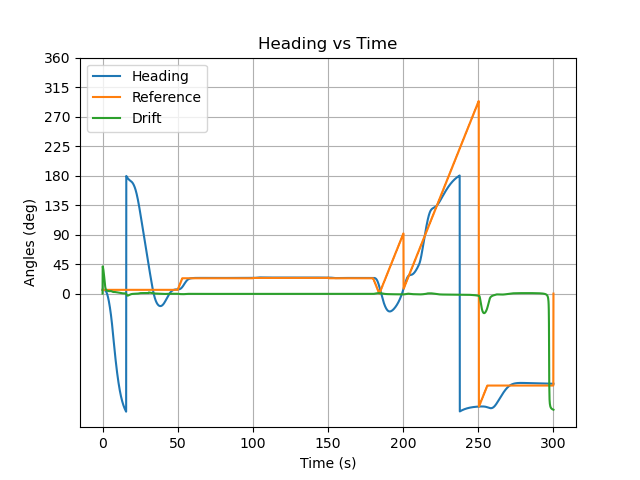
\includegraphics[trim={0.5cm 0.25cm 1.25cm 0.75cm },clip]{documents/final_pres_figs/with_wind_to_40_40_heading.png}
    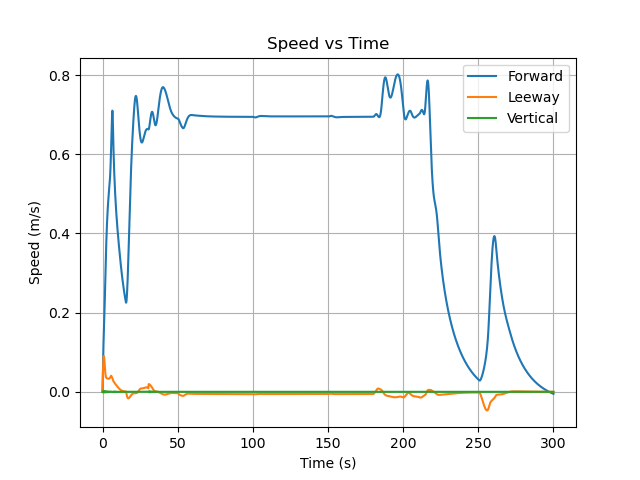
\includegraphics[trim={0.5cm 0.25cm 1.25cm 0.75cm },clip]{documents/final_pres_figs/with_wind_to_40_40_speed.png}
    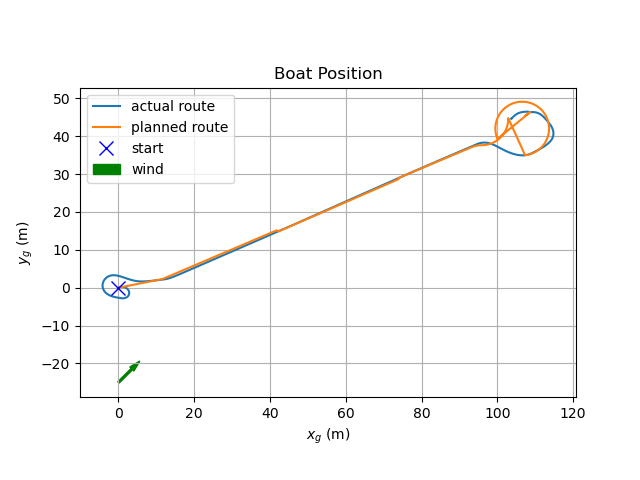
\includegraphics[trim={0.5cm 1cm 1.25cm 1.5cm },clip]{documents/final_pres_figs/with_wind_to_40_40_pos.png}
    \caption{Sailing with wind: sailing to \((x,y) = (100,40)\) with wind in the direction of sailing. No waves.}
    \label{fig:sail_with_wind}
\end{figure}

\begin{figure}
    \centering
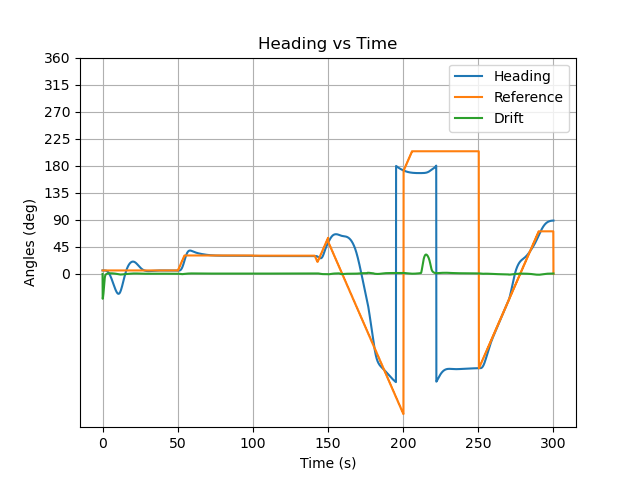
\includegraphics[trim={0.5cm 0.25cm 1.25cm 0.75cm },clip]{documents/final_pres_figs/right_to_wind_to_40_40_heading.png}
         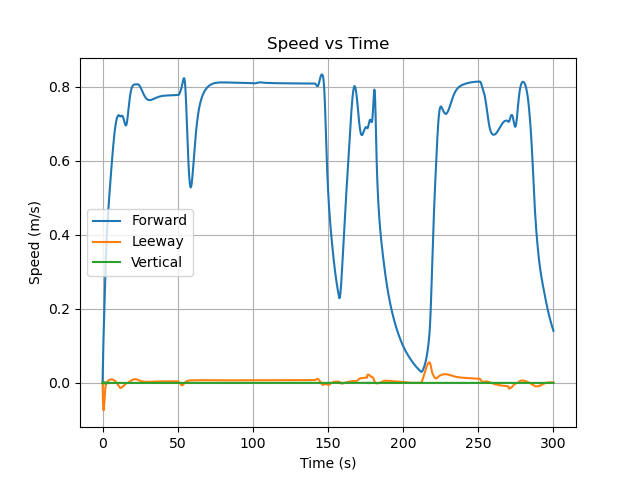
\includegraphics[trim={0.5cm 0.25cm 1.25cm 0.75cm },clip]{documents/final_pres_figs/right_to_wind_to_40_40_speed.png}
                  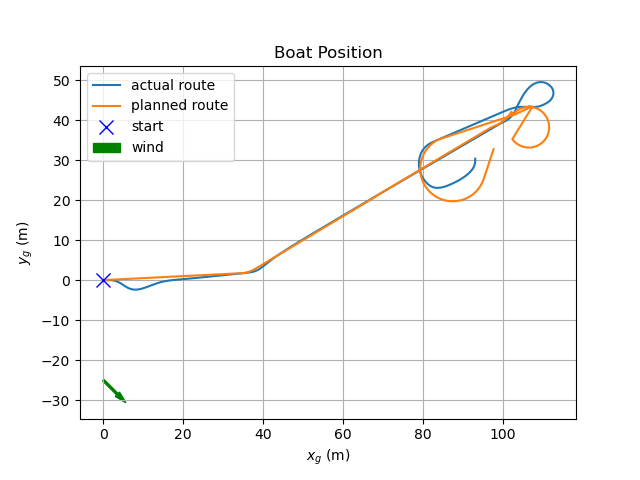
\includegraphics[trim={0.5cm 0.25cm 1.25cm 0.75cm },clip]{documents/final_pres_figs/right_to_wind_to_40_40_pos.png}
    \caption{Sailing with crosswinds: sailing to \((x,y) = (100,40)\) with with crosswinds. No waves.}
    \label{fig:sail_right_wind}
\end{figure}


\begin{figure}
     \centering
     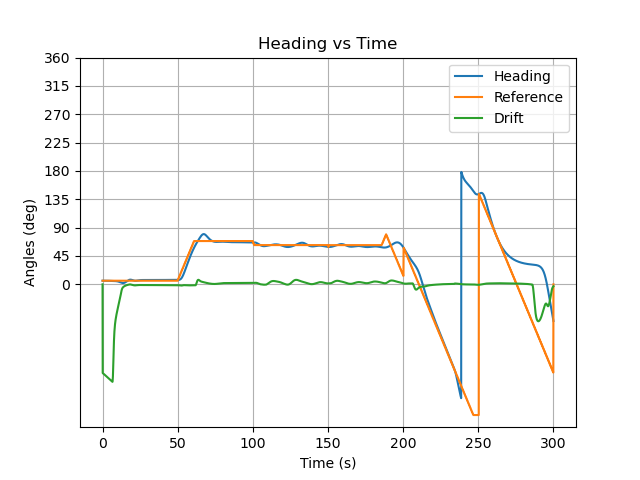
\includegraphics[trim={0.5cm 0.25cm 1.25cm 0.75cm},clip]{documents/final_pres_figs/against_wind_to_40_40_heading.png}
     
     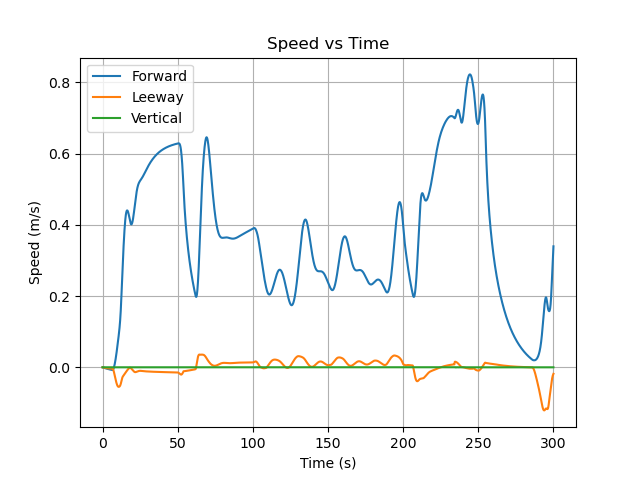
\includegraphics[trim={0.5cm 0.25cm 1.25cm 0.75cm },clip]{documents/final_pres_figs/against_wind_to_40_40_speed.png}
     
     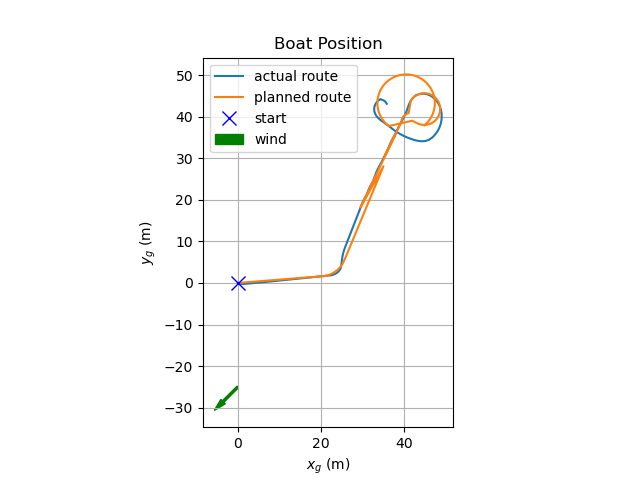
\includegraphics[trim={0.5cm 0.0cm 1.25cm 0.5cm },clip]{documents/final_pres_figs/against_wind_to_40_40_pos.png}
     
    \caption{Sailing against the wind: sailing to \((x,y)=(40,40)\) with the winds against direction of sailing. No waves.}
    \label{fig:sail_against_wind}
\end{figure}


\begin{figure}
\centering
    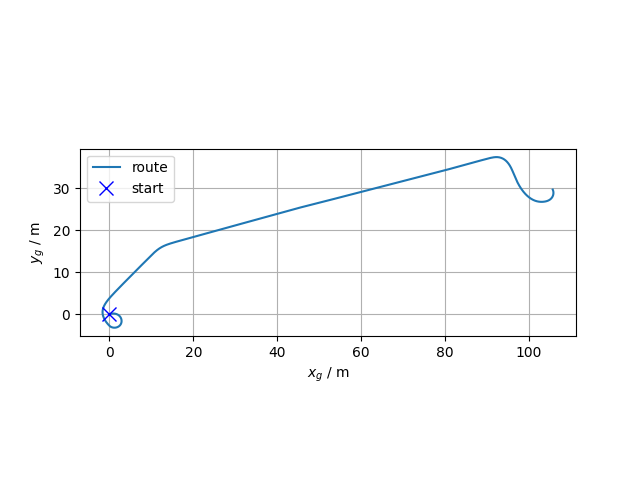
\includegraphics[trim={0.5cm 2cm 1.5cm 2.5cm},clip]{Figures/no-obstacle-no-waves-wind-5-10/position.png}
    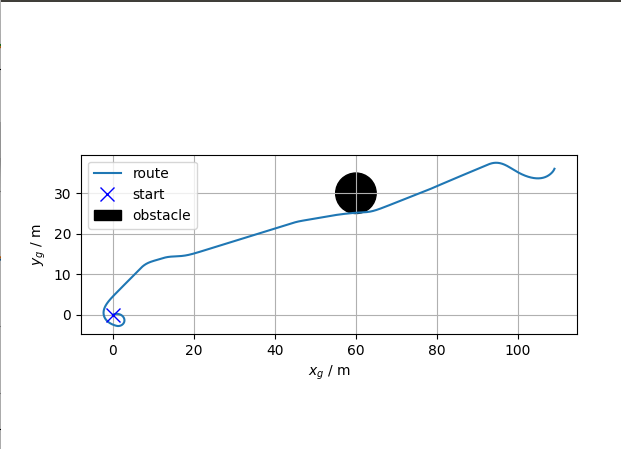
\includegraphics[trim={0.5cm 2cm 1.25cm 2.5cm},clip]{Figures/Obstacles-waves-wind-4-45/obsta.png}
    \caption{Single obstacle avoidance to reach \((100, 40)\) with wind in the direction of sailing and no waves.}
    \label{fig:no_wind_one_obs}
\end{figure}

\begin{figure}
    \centering
         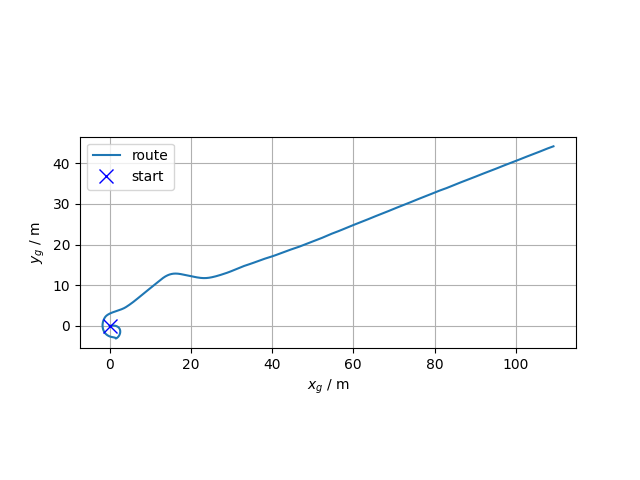
\includegraphics[trim={0.5cm 2cm 1.25cm 2.5cm},clip]{Figures/no-obstacle-waves-wind-5-65/position.png}
         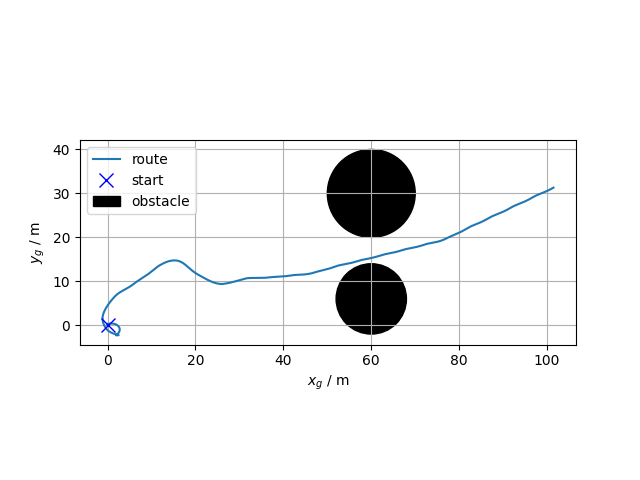
\includegraphics[,trim={0.5cm 2cm 1.25cm 2.5cm},clip]{Figures/Obstacles-waves-wind-4-45/position-(with-waves).png}
    \caption{Channel navigation to reach \((100, 40)\) with wind in the direction of sailing and \SI{0.5}{\meter} waves}
    \label{fig:with_wind_channel}
\end{figure}

\section{Discussion}

On these experiments, the boat tracks well the planned trajectory computed against the simplified boat model. The plans clearly demonstrate look-ahead capability on the experiments with boats, and also in planning loops around the target position. Note that the boat model is not drift free, so the planner must plan a trajectory which keeps the boat near the target once the boat reaches the target.

However, as can be seen in Figure \ref{fig:sail_against_wind} where the planned route in orange jogs bag several meters around \((x,y) = (30,20)\), the constant speed assumption of the simplified boat model begins to be severely limited when facing into the wind. The boat goes slower than expected so the replanning must account for that.  

The planner, with the parameters as given, usually completes a plan in 1-5 seconds. However, there are some cases where it can take upwards of 30 seconds. The cause of these spikes in computation time is currently unknown.


\section{Conclusion}
We have demonstrated a method for path planning and obstacle avoidance of a sailboat using an optimization-based planner. The planner is flexible enough to allow the sailboat to traverse a channel and avoid obstacles under different environmental conditions, such as different wind directions and the presence of waves.

Although we used the \Sim for simplicity, we encountered several of its limitations. The simulator uses a constant wind vector, so we were unable to test gusts of wind. Robustness to extreme weather, such as high winds, would be another goal. Successfully traversing a narrow channel with high winds would be challenging, especially if the wind were not steady.


% \section{Future Work}
% The \Sim has some limitations. Foremost is that has not been verified to accurately model real-world sailing. In terms of environmental disturbances, it does not support varying wind. We were not able to try wind gusts and strange water currents. Additionally, more testing would be helpful. More conditions, different sized boats, moving obstacles.

\bibliographystyle{IEEEtran}
\bibliography{refs.bib}
\end{document}